\documentclass{wx672article} % $HOME/texmf/tex/latex/wx672article.cls

\usepackage{wx672cjk}
\usepackage[NoDate]{currvita}

\newlength{\outerbordwidth}
\pagestyle{empty}
\raggedbottom
\raggedright
%\usepackage[svgnames]{xcolor}
\usepackage{framed}
\usepackage{tocloft}



%-----------------------------------------------------------
%Edit these values as you see fit

\setlength{\outerbordwidth}{3pt}  % Width of border outside of title bars
\definecolor{shadecolor}{gray}{0.75}  % Outer background color of title bars (0 = black, 1 = white)
\definecolor{shadecolorB}{gray}{0.93}  % Inner background color of title bars


%-----------------------------------------------------------
%Margin setup

\setlength{\evensidemargin}{-0.25in}
\setlength{\headheight}{0in}
\setlength{\headsep}{0in}
\setlength{\oddsidemargin}{-0.25in}
\setlength{\paperheight}{11in}
\setlength{\paperwidth}{8.5in}
\setlength{\tabcolsep}{0in}
\setlength{\textheight}{9.5in}
\setlength{\textwidth}{7in}
\setlength{\topmargin}{-0.3in}
\setlength{\topskip}{0in}
\setlength{\voffset}{0.1in}


%-----------------------------------------------------------
%Custom commands
\newcommand{\resitem}[1]{\item #1 \vspace{-2pt}}
\newcommand{\resheading}[1]{\vspace{8pt}
  \parbox{\textwidth}{\setlength{\FrameSep}{\outerbordwidth}
    \begin{shaded}
\setlength{\fboxsep}{0pt}\framebox[\textwidth][l]{\setlength{\fboxsep}{4pt}\fcolorbox{shadecolorB}{shadecolorB}{\textbf{\sffamily{\mbox{~}\makebox[6.762in][l]{\large #1} \vphantom{p\^{E}}}}}}
    \end{shaded}
  }\vspace{-5pt}
}
\newcommand{\ressubheading}[4]{
\begin{tabular*}{6.5in}{l@{\cftdotfill{\cftsecdotsep}\extracolsep{\fill}}r}
		\textbf{#1} & #2 \\
		\textit{#3} & \textit{#4} \\
\end{tabular*}\vspace{-6pt}}
%-----------------------------------------------------------


\begin{document}
\begin{cv}{Qiyuan Pu}
  \vspace*{-1ex}
  {\small I can write a simple operating system}\\[2ex]
  \begin{tabular}{r@{\,:\,}l}%
    {\scriptsize\fa }&\emph{pqy7172@gmail.com} \\%
    {\fa }&\emph{+86 18314555392}\\%
    
  \end{tabular}


  
  \vspace*{\dimexpr-1.5in-\topmargin-\headsep-\headheight-\baselineskip}%
  \hspace*{\dimexpr-1in-\evensidemargin-\parindent}%
  \hspace*{-10ex}
  \makebox[\paperwidth][r]{\frame{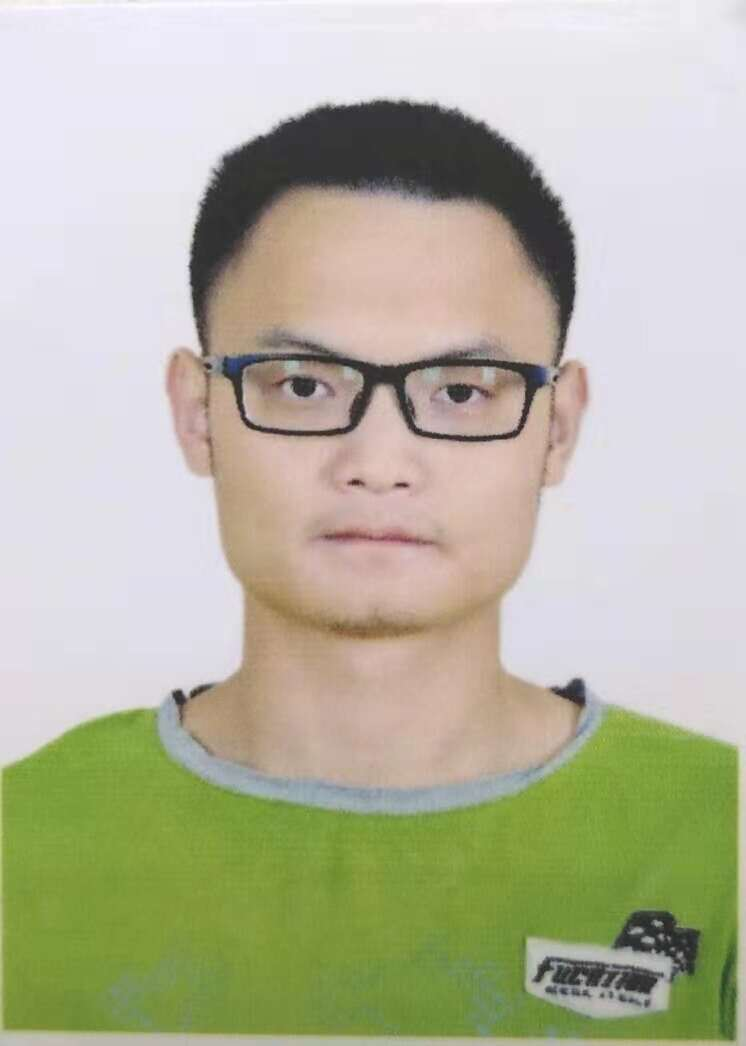
\includegraphics[width=0.15\textwidth]{me3}}}

  

    
  \begin{cvlist}{Education Background}
  \item[09/2014 -- 06/2018] Southwest Forestry University, School of Big Data and
    Intelligent Engineering, Computer Science and Technology, Bachelor
    \begin{itemize}
    \item Majored Course: Data Structure, Operating System, Computer Architecture,
      Computer Network, etc. These major courses are all 90 points or more, out of 100.
    \item In the third semester, I went to Thailand as a school exchange student.
    \end{itemize}
  \end{cvlist}

  \begin{cvlist}{Development Experience}
  \item[RongOS --- Implementation of a simple operating system]\ \par
    This project has written a simple operating system from scratch. Implemented features
    include multitasking, memory management, process management, windows management,
    etc. This project is also my graduation design and won the Outstanding Graduation
    Thesis Award.
    \begin{itemize}
    \item \url{https://github.com/Puqiyuan/RongOS}
    \item \url{https://github.com/Puqiyuan/RongOS/blob/master/doc/thesis/thesis.pdf}
    \end{itemize}
  \item[Tsinsen Website Programming Challenge] \ \par
    This project is to independently complete the Tsinsen problems to train programming
    skills. The problems currently completed are all 100 scores, out of 100. There are
    other similar exercises, including two C programs, one is high-precision (up to 999 digits
    before and after the decimal point) floating-point calculator, the other is banker
    algorithm in the operating system, etc., basically representing my current highest
    programming ability.
    \begin{itemize}
    \item \url{https://github.com/Puqiyuan/Tsinsen_ACM}
    \item \url{https://github.com/Puqiyuan/URI_ACM}
    \item
      \url{https://github.com/Puqiyuan/High_Accuracy_Float_Calculator/blob/master/Calculator.c}
    \item
      \url{https://github.com/Puqiyuan/OS_Algorithms/blob/master/BankerAlgorithm/Programs/banker.c}
    \end{itemize}
  \item[Advanced Programming in the UNIX Environment] \ \par
    Includes files, directories, standard I/O, system data files and information, process
    environment, process control, process relationships, signals, threads, thread control,
    daemons, process communication, network IPC, and more. C development under Linux is
    the direction I want to pursue, and the future professional expectation is Linux
    system/background development, and it is best to involve the kernel.
    \begin{itemize}
    \item \url{https://github.com/Puqiyuan/APUE}
    \end{itemize}
  \end{cvlist}
  \begin{cvlist}{Self-evaluation}
  \item[] Through the university for four years, a series of excellent study, work and
    living habits havebeen developed, including:
    \begin{enumerate}
    \item Skilled in using Google English search to solve various problems, English is my working language.
    \item Efficient command line work manner.
    \item Skilled in using Linux tools, including Emacs, Vim, Latex, Org-Mode,
      Makefile, Github, etc.
    \item Skilled C programming, with three years of experience in Debian Linux
      configuration, a certain Bash Shell programming experience, a certain understanding
      of C development under Linux.
    \item Persist in running ten or twenty kilometers a week. Patience and perseverance
      are decisive for the resolution of technical problems.
    \end{enumerate}
  \end{cvlist}
  \begin{cvlist}{Personal Honor}
  \item[2014 — 2015] Merit Student in University Level
  \item[2015 — 2016] Merit Student in Province Level
  \item[2018] Outstanding Graduate
  \item[2018] Excellent Graduation Thesis(Design)
  \item[2018] Second Prize of Yunnan Province University Students Computer Works
    Competition
  \end{cvlist}
\end{cv}
\end{document}








%%% Local Variables:
%%% mode: latex
%%% TeX-master: t
%%% End:
